\squarebox[LightBlue]{
\chapterabstract{This chapter presents a novel approach for identifying network issues in Cloud VR sessions over Wi-Fi networks. It introduces a two-stage framework that combines contrastive anomaly detection with supervised classification to detect and diagnose performance impairments. The chapter recalls the design of a controlled Wi-Fi testbed used to collect time series KPIs, which serve as the basis for evaluating the proposed model. Extensive empirical experiments compare the solution against state-of-the-art time series classification models, demonstrating its effectiveness, even in low-label scenarios. Additionally, the chapter highlights the model's suitability for real-time deployment due to its balance between training efficiency and inference speed.}}

\minitoc


\section{Introduction}\label{chap_6:introduction}
The recent evolution of network technologies has led to the rise of low-latency applications such as cloud gaming, telemedicine, cloud robotics, and cloud virtual reality (VR). Cloud VR eliminates the need for powerful local processing hardware by offloading computation to remote servers, enabling the use of lightweight and cost-effective VR headsets. This architecture opens avenues for diverse innovations, including immersive gaming experiences, enhanced virtual collaboration, and advanced training simulations across various domains. Cloud VR has particularly gained significant importance in recent years \cite{nextmscVirtualReality} due to its ability to deliver immersive, high-resolution VR content to end-users. Cloud VR applications, however, come with stringent technical requirements. They typically require high-resolution content streaming (up to 4K-8K) with high bandwidth demands ($\geq 80$ Mbps) and ultra-low latency ($\leq 20$ ms) to ensure a seamless and interactive user experience. Meeting these requirements is essential to avoid issues like lag, reduced interactivity, and user discomfort, which can culminate in cybersickness \cite{huawei}.  

These demanding requirements pose significant challenges for Cloud VR applications when delivered over wireless networks, particularly Wi-Fi networks. Although recent Wi-Fi standards (e.g., Wi-Fi 6) enable higher bandwidth and lower latency under ideal line-of-sight conditions, real-world performance is hindered by several limitations. These include bandwidth variability, jitter, additional latency, and packet loss, which are exacerbated by environmental factors such as 1) signal attenuation that occurs due to obstacles that absorb the Wi-Fi signal (e.g., walls, furniture); 2) interference that may arise from nearby access points (APs) or coexisting IoT devices using Wi-Fi or Bluetooth protocols, particularly in dense urban environments; or 3) network congestion that can result from high traffic loads on the same AP or simultaneous access by multiple users. These factors degrade the \ac{QoE} for end-users, causing delays, black-edge events, or poor synchronization between movements and visuals, all of which undermine the immersive nature of VR applications \cite{li2020performance, lee2024adaptive, rossi2024subjective}

Given the growing importance of Cloud VR applications, it is imperative to detect and diagnose  performance degradation issues to ensure consistent and reliable sessions. Accurate root-cause diagnosis can help improve network architectures to support emerging low-latency applications or enable \ac{ISP}) to develop intelligent APs capable of diagnosing and mitigating impairments dynamically. Traditionally, root-cause diagnosis has been performed using expert-based rules \cite{hochenbaum2017automatic, chen2019matrix}. In this approach, network experts analyze \ac{KPIs} using predefined heuristics, thresholds, or conditions to identify anomalies and determine their root causes. While effective in simple scenarios, this method is manual, time-consuming, and does not scale well to modern, complex network environments where vast amounts of KPIs are generated continuously.  

In recent years, advancements in machine learning (ML) have revolutionized root-cause diagnosis by automating the analysis of large-scale KPI data. Machine learning models can automatically process time-series KPI data to perform root-cause diagnostic efficiently. \ac{TSC} techniques, in particular, have emerged as effective tools for this task, as they can capture temporal patterns and relationships essential for identifying each cause. Several categories of TSC techniques have been proposed, including distance-based (e.g., DTW), kernel-based (e.g., SVM), shapelet-based approaches, tree-based algorithms or deep learning models leveraging MLPs, CNNs, RNNs, and GNNs \cite{ismail2019deep, faouzi2022time,mohammadi2024deep}. However, supervised TSC methods rely on annotated datasets, which are often expensive and time-consuming to generate, as they require domain expertise to label vast amounts of KPI data. To address the challenges of annotation, researchers are increasingly shifting toward \ac{SSL} for unsupervised time-series classification. SSL has achieved remarkable performance in fields like computer vision and \ac{NLP} by learning meaningful representations of data without relying on labeled samples. Unlike supervised methods, self-supervised approaches define pretext tasks (e.g., contrastive learning or self-prediction) to extract underlying features from raw data. One of the most popular SSL frameworks is \ac{CL}, which uses data augmentation to generate multiple views from a single instance. Positive pairs (augmented views of the same instance) are brought closer together in the feature space, while negative pairs (views of different instances) are pushed apart. Contrastive learning has demonstrated significant success in representation learning for time-series data and forms the foundation of many state-of-the-art unsupervised TSC methods.  

Inspired by these advancements, we propose \ac{RAID}, a two-stage machine learning framework for root-cause diagnosis of performance degradation in Cloud VR applications over Wi-Fi networks: in the first stage, an anomaly detection model uses contrastive learning to differentiate between normal and anomalous time-series KPIs. In the second stage, a lightweight supervised classifier that distinguishes between different types of anomalies detected in Stage 1. We empirically demonstrate that this two-stage framework outperforms existing competing methods, even when trained with limited labeled data. The evaluations are conducted on KPI datasets collected from the real-world Cloud VR testbed, presented on Chapter \ref{chap:measurements}, featuring a Cloud VR application built on NVIDIA CloudXR architecture. The system streams VR content over a Wi-Fi connection using a commercial access point and an Oculus Quest 2 headset. Our proposed solution offers a scalable and efficient method for root-cause diagnosis, paving the way for improved network support for low-latency applications like Cloud VR.  

\contributions{
Specifically, the key contributions of this chapter are as follows:
\begin{itemize}
    % \item We design a controlled Wi-Fi testbed that replicates real-world network impairments, enabling the study of their impact on Cloud VR performance.
    \item We introduce a novel two-stage framework that combines contrastive learning-based anomaly detection with supervised classification to effectively detect and diagnose Wi-Fi impairments in Cloud VR environments.
    \item We perform extensive empirical evaluations using time series KPI datasets collected from our testbed that replicates real-world network impairments, comparing our proposed solution with state-of-the-art time series classification models.
    \item Our solution demonstrates strong performance even in low-label scenarios, highlighting its ability to generalize with minimal supervision. Additionally, it offers a balanced trade-off between moderate training time and low inference latency, making it well-suited for real-time deployment in practical applications.
\end{itemize}
}


\section{Related work}\label{chap_6:related_work}
\subsection{ML-based network root cause diagnosis}

\ac{RCD} aims to identify the underlying reasons behind network anomalies, such as degraded performance or failures. The advent of machine learning (ML) has driven the development of numerous data-driven solutions for RCD, leveraging ML models to analyze network data and pinpoint the sources of issues. Below, we discuss notable research efforts in this domain, focusing on various supervised and unsupervised techniques tailored for network environments.

Dimopoulos et al. \cite{dimopoulos2015identifying} introduced a supervised ML framework to detect the root cause of QoE issues in video streaming. The metrics were collected from three key vantage points—mobile devices, routers, and content servers—to train supervised models. This work highlights the effectiveness of incorporating diverse data sources in diagnosing video streaming issues, enabling targeted interventions.
Kawasaki et al. \cite{kawasaki2020comparative} focused on root cause analysis in \ac{NFV} environments. The study applied supervised ML algorithms such as MLP, SVM, and Random Forests for fault classification. By comparing multiple ML models, the authors demonstrate the feasibility of using supervised approaches for diagnosing issues in complex, virtualized networks.
Salik et al. \cite{salik2023non} detected non-WiFi interference and estimated its impact on WiFi throughput for both 2.4GHz and 5GHz bands. The authors developed supervised models, including Random Forest, CatBoost, and MLP, using network metrics collected at the WiFi edge. This approach effectively identified and mitigated interference from non-WiFi sources, improving network reliability in congested environments.
Syrigos et al. \cite{syrigos2019employment} developed ML-based tools to troubleshoot common WiFi impairments such as contention, interference, hidden terminals, and low signal strength. Supervised ML models were trained on curated datasets to classify network impairments, enabling actionable diagnostics. The framework provided a systematic way to enhance WiFi network performance by pinpointing specific issues.
Dötterl et al. \cite{dotterl2024classification} classified home network problems using advanced deep learning techniques. A transformer-based architecture is employed to analyze outputs from network monitoring tools like ping and dig. It demonstrated that transformer models can effectively classify complex network problems, offering precise diagnostics for home networks.

Fida et al. \cite{fida2023bottleneck} proposed a two-stage framework for bottleneck identification in cloudified 5G networks: in Stage 1, an unsupervised \ac{VAE} detects anomalies in network telemetry data while in Stage 2, an MLP classifier identifies the specific root cause of the bottlenecks. The distributed telemetry framework enabled real-time diagnosis in 5G networks, demonstrating scalability and adaptability in modern mobile environments.

Our work builds on recent advancements in \ac{RCD} by addressing the limitations of existing solutions that rely exclusively on supervised methods. We introduce a novel approach specifically tailored for low-latency applications operating in Wi-Fi network environments. By leveraging contrastive learning, our solution enhances diagnostic accuracy, particularly in scenarios with limited labeled data. While our approach shares similarities with the method proposed in \cite{fida2023bottleneck}, we differentiate ourselves by employing contrastive learning for anomaly detection, which results in improved performance.

% Zhao et al. \cite{zhao2024fault} introduced a graph-based convolutional network (GCN) method for 5G networks, leveraging user-side KPIs and synthetic data generated by GANs. Their approach also incorporated expert-based correlation graphs to enhance model training and interpretability

% Zhang et al. \cite{zhang2018wifi} WiFi and Multiple Interfaces: Adequate for Virtual Reality? 
% Burbano et al. \cite{burbano2024impact} Impact of Network Factors on QoE-sensitive Virtual Reality Environments: An Experimental Analysis Perspective using VR-based Mindfulness

\subsection{Time series Classification}
\ac{TSC} has been a prominent research topic for decades due to its applicability in numerous real-world domains, including cybersecurity and network management. A variety of solutions have been proposed in the literature, with methods ranging from classical approaches to modern deep learning techniques.

According to Bagnall et al. \cite{bagnall2017great}, classical TSC methods can be categorized into several groups including distance-based methods amoung those one of the most prominent examples is the 1-NN-DTW algorithm, which performs one-nearest-neighbor classification using dynamic time warping (DTW) as the distance metric; interval-based methods like Time Series Forest (TSF) \cite{deng2013time} which leverage random forests and extract summary statistics from intervals of time series data to improve classification accuracy; shapelet-based methods like binary shapelet transformation methods \cite{bostrom2015binary} which use shapelets that are phase-independent subseries that capture discriminative patterns within time series data for TSC or ensemble-based methods like Collective of Transformation-based Ensembles (COTE) \cite{bagnall2015time} that combines classifiers trained on different data representations. This approach highlights the importance of transforming data into subspaces where features are more easily discriminable.

In recent years, deep learning techniques have gained significant traction in TSC due to their ability to learn complex and hierarchical features directly from raw data. Various architectures have been proposed, including MLPs, CNNs, TCNs or RNNs \cite{zheng2016exploiting, wang2017time, zhao2017convolutional}. These techniques were supervised learning techniques and were successful in time series classification over diverse domains \cite{ismail2019deep}. However, the rise of SSL have come with a jump in performance of TSC models. In fact, SSL has gained significant interest for its ability to learn meaningful representations from unlabeled data through carefully designed pretext tasks on computer vision or natural language processing. These tasks aim to uncover the intrinsic structure of the data, enabling the learned representations to be effectively utilized in downstream tasks, including TSC. Among the various SSL approaches, CL has emerged as particularly effective. It works by encouraging similar samples (positive pairs) to cluster in the feature space while pushing apart dissimilar samples (negative pairs). For time series data, numerous CL frameworks have been proposed, demonstrating strong performance on TSC tasks. T-Loss \cite{franceschi2019unsupervised} introduces a triplet loss that constructs positive pairs using subseries extracted from the same time series, while negative pairs are formed using subseries from other time series. Coupled with a SVM, the learned representations perform exceptionally well on multivariate TSC tasks, demonstrating robust feature extraction. TNC (Temporal Neighborhood Coding) \cite{tonekaboni2021unsupervised} constructs pairs based on the concept of temporal neighborhoods, leveraging statistical tests to identify segments of a time series that share similar underlying properties. It achieves excellent results on simulated and real-world datasets, such as ECG data, by capturing temporal dependencies. TS-TCC (Time-Series Temporal and Contextual Contrastive Learning) \cite{Eldele2021TimeSeriesRL} employs cross-view prediction using data augmentations and integrates temporal and contextual contrastive learning modules. This design ensures the model learns robust, discriminative representations and demonstrates superior accuracy on TSC tasks across diverse domains by effectively handling temporal dynamics. CLOCS \cite{kiyasseh2021clocs} specifically designed for ECG signals, applies data transformations to learn patient-specific representations that are invariant to spatio-temporal variations. Focused on healthcare, this method excels in classifying ECG time series by capturing unique and invariant features. TF-C (Time-Frequency Contrastive Framework) \cite{zhang2022self} encourages time series with time and frequency similarity to cluster in the time-frequency space thanks to the introduction of novel frequency-based augmentation techniques to generate augmented views of the data. It achieves competitive results in TSC across a wide range of domains, showcasing the effectiveness of incorporating frequency-domain information. TS2Vec \cite{Yue2021TS2VecTU} proposes a hierarchical framework to learn both temporal-wise and instance-wise similarities at multiple semantic levels. The contextual consistency-based pair selection enhances representation learning for diverse time series patterns. It demonstrates versatility and efficiency in multivariate TSC and other related tasks, further establishing the value of contextual representation learning.

We tackle RCD in Cloud VR as a time series classification problem. Unlike aforementioned approaches to time series classification, our method employs a two-stage framework: first, it identifies normal scenario time series, and then it classifies faulty scenarios, thereby improving the overall accuracy and effectiveness of the classification process.


 

% \subsection{Anomaly detection techniques}

% Anomaly detection (AD) has been extensively studied, with methods broadly categorized into machine learning and deep learning based approaches. Traditional statistical methods assume that anomalies deviate from high-probability regions of a probabilistic model. Parametric methods like ARIMA \cite{yaacob2010arima} and Gaussian-based techniques \cite{luo2017gas} rely on specific distributions, while non-parametric methods, such as \ac{KDE} \cite{cao2016one}, estimate density functions without such assumptions. Distance-based methods, including k-Nearest Neighbors (kNN) \cite{chaovalitwongse2007time} and \ac{LOF} \cite{breunig2000lof}, identify anomalies by measuring distances or densities in feature space. Additionally, spectral analysis methods like Principal Component Analysis (PCA) \cite{paffenroth2018robust} and isolation-based techniques like Isolation Forest (IF) \cite{liu2008isolation} are commonly used for AD.  

% Deep learning methods have significantly advanced AD, particularly in complex time series and high-dimensional data. Reconstruction-based techniques, such as autoencoders (AEs), detect anomalies by measuring reconstruction errors. Advanced models like VAEs \cite{xu2018unsupervised} and DAGMM \cite{zong2018deep} combine probabilistic models and dimensionality reduction for improved performance. Temporal dependencies are captured using RNN-based methods like LSTM-VAE \cite{park2018multimodal} and Omni-Anomaly \cite{su2019robust}, while Transformer-based models such as Anomaly Transformer \cite{xu2022anomaly} and TranAD \cite{tuli2022tranad} leverage attention mechanisms for long-sequence AD. Generative models, including GAN-based frameworks like MAD-GAN \cite{li2019mad} and BeatGAN \cite{zhou2019beatgan}, focus on reconstructing time series data while adversarially training models to enhance robustness. Forecasting-based methods, such as LSTM-PRED \cite{goh2017anomaly} and Telemanom \cite{hundman2018detecting}, use deviations between predicted and observed values for anomaly identification.  

% Recent advancements in contrastive learning have further improved AD performance by enhancing representation learning. Frameworks like COCA \cite{wang2023deep} and ContrastAD \cite{li2023contrastive} leverage contrastive losses to train models on positive and negative pairs, with techniques like data augmentation and synthetic anomaly generation enriching the training process. CARLA \cite{DARBAN2025110874} combines self-supervised learning with contrastive loss to distinguish normal and anomalous samples effectively, while DCdetector \cite{yang2023dcdetector} employs multi-scale attention mechanisms to capture spatial and temporal dependencies. These approaches highlight the evolution of AD from traditional statistical methods to advanced DL techniques, emphasizing the growing importance of representation learning and model adaptability in diverse application scenarios.  

% Our work leverages anomaly detection techniques as a foundational step in our two-stage framework for RCD, aiming to improve classification accuracy. Similar to prior studies, we incorporate contrastive learning to enhance the representation of both anomalous and normal time series. This approach not only strengthens the detection of anomalies but also significantly improves the performance of the subsequent classification task, setting our method apart in effectively addressing RCD challenges.


% \section{Testbed}\label{chap_6:testbed}
% This section outlines the testbed developed for CloudVR experiments, which leverages the NVIDIA CloudXR architecture to deliver immersive virtual reality experiences over wireless networks. We begin by providing an overview of the CloudVR application framework, followed by a detailed description of the testbed infrastructure and automation components.

\subsection{Testbed Infrastructure}

The testbed is built upon the NVIDIA CloudXR SDK, an \ac{XR} streaming platform that utilizes edge computing and cloud-based GPU acceleration to deliver high-fidelity VR experiences. The CloudXR platform streams OpenVR-based applications from a remote server to XR client devices with limited graphical capabilities, such as the untethered \ac{HMDs} Meta Quest 2 and Meta Quest 3. These devices connect to the server through various network interfaces, including Ethernet, Wi-Fi, or cellular connections.

The CloudXR architecture comprises a server-side driver responsible for streaming audio and video content from XR applications (e.g., SteamVR) to the client device using network protocols like UDP; a client-side software that enables the HMD to receive and render streamed VR content, ensuring low-latency interactions and maintaining high-quality visuals.

The CloudVR testbed, as depicted in Fig. \ref{fig:chap_6:testbed}, facilitates controlled experiments under realistic network conditions. The testbed consists of a server (a machine with an Intel Xeon W2235 CPU @ 3.8GHz, 32 GB of RAM, and an NVIDIA GeForce RTX 3090 Ti GPU) running the CloudXR server software to render and stream VR content; a client (Meta Quest 2 HMD) wirelessly connected to the network and a Wi-Fi \ac{AP} (here a Orange Livebox router).

\begin{figure*}[!ht]
    \centering
    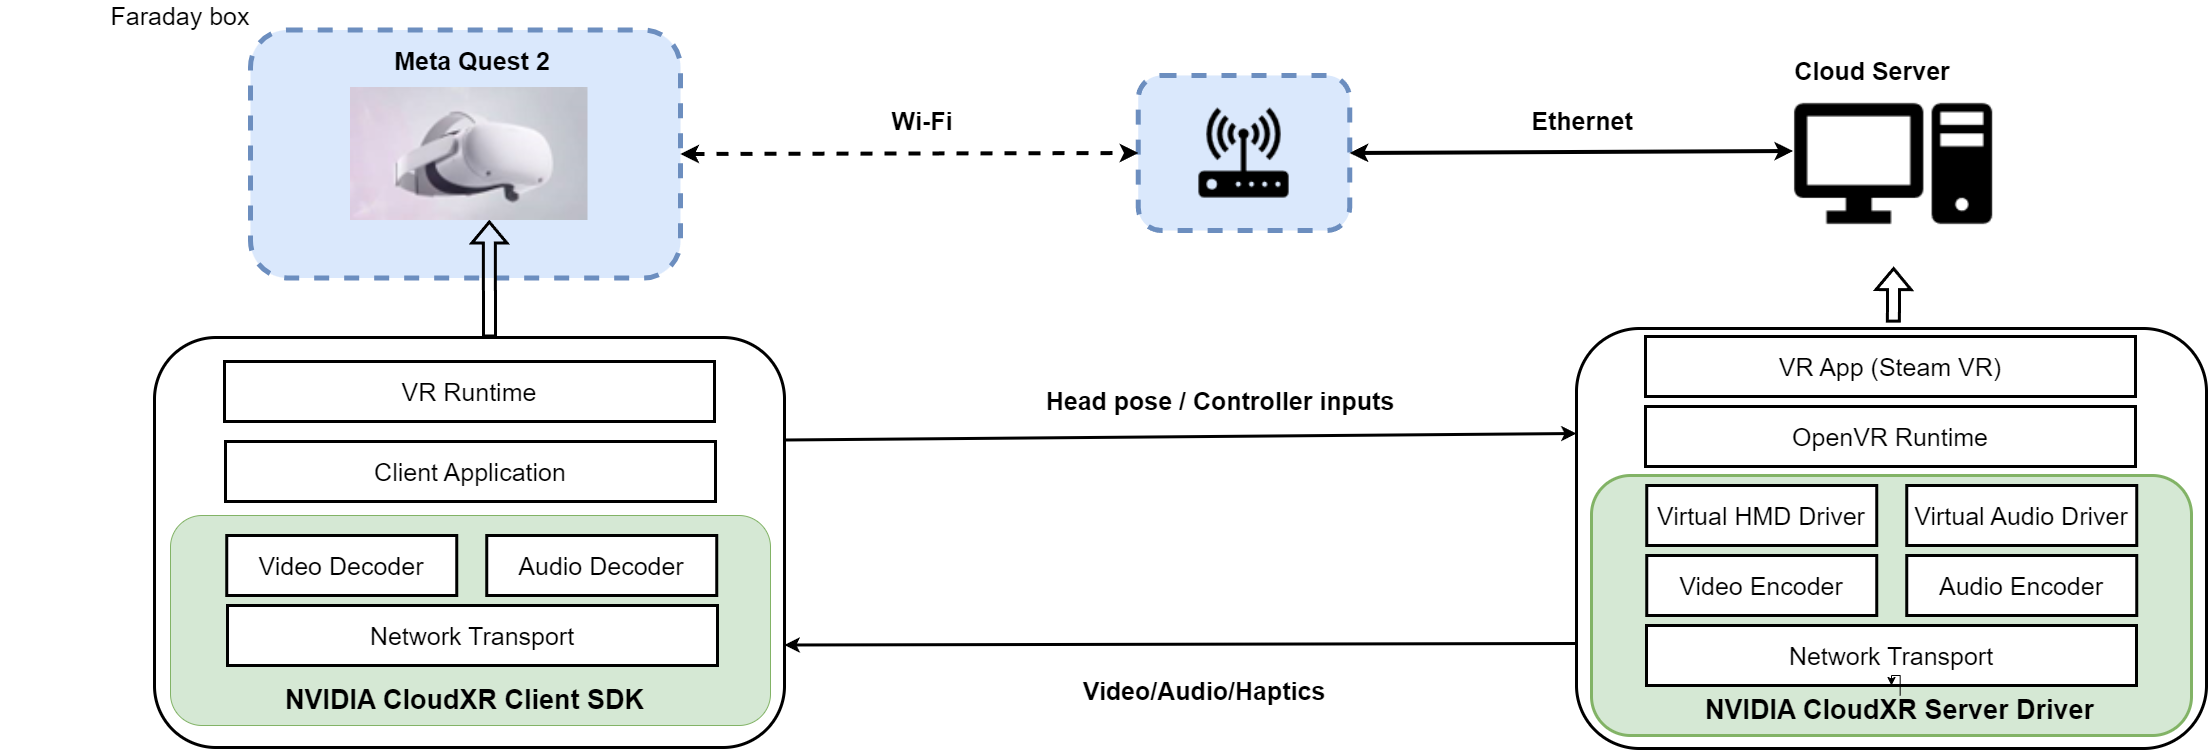
\includegraphics[width=\linewidth]{imgs/chapter_6/cloud_xr_stack.png}
    \caption{Cloud VR testbed}
    \label{fig:chap_6:testbed}
\end{figure*}


%-------------------description of FA testbed (Minqi Nicolas)--------------------

\begin{figure*}[!ht]
    \centering
    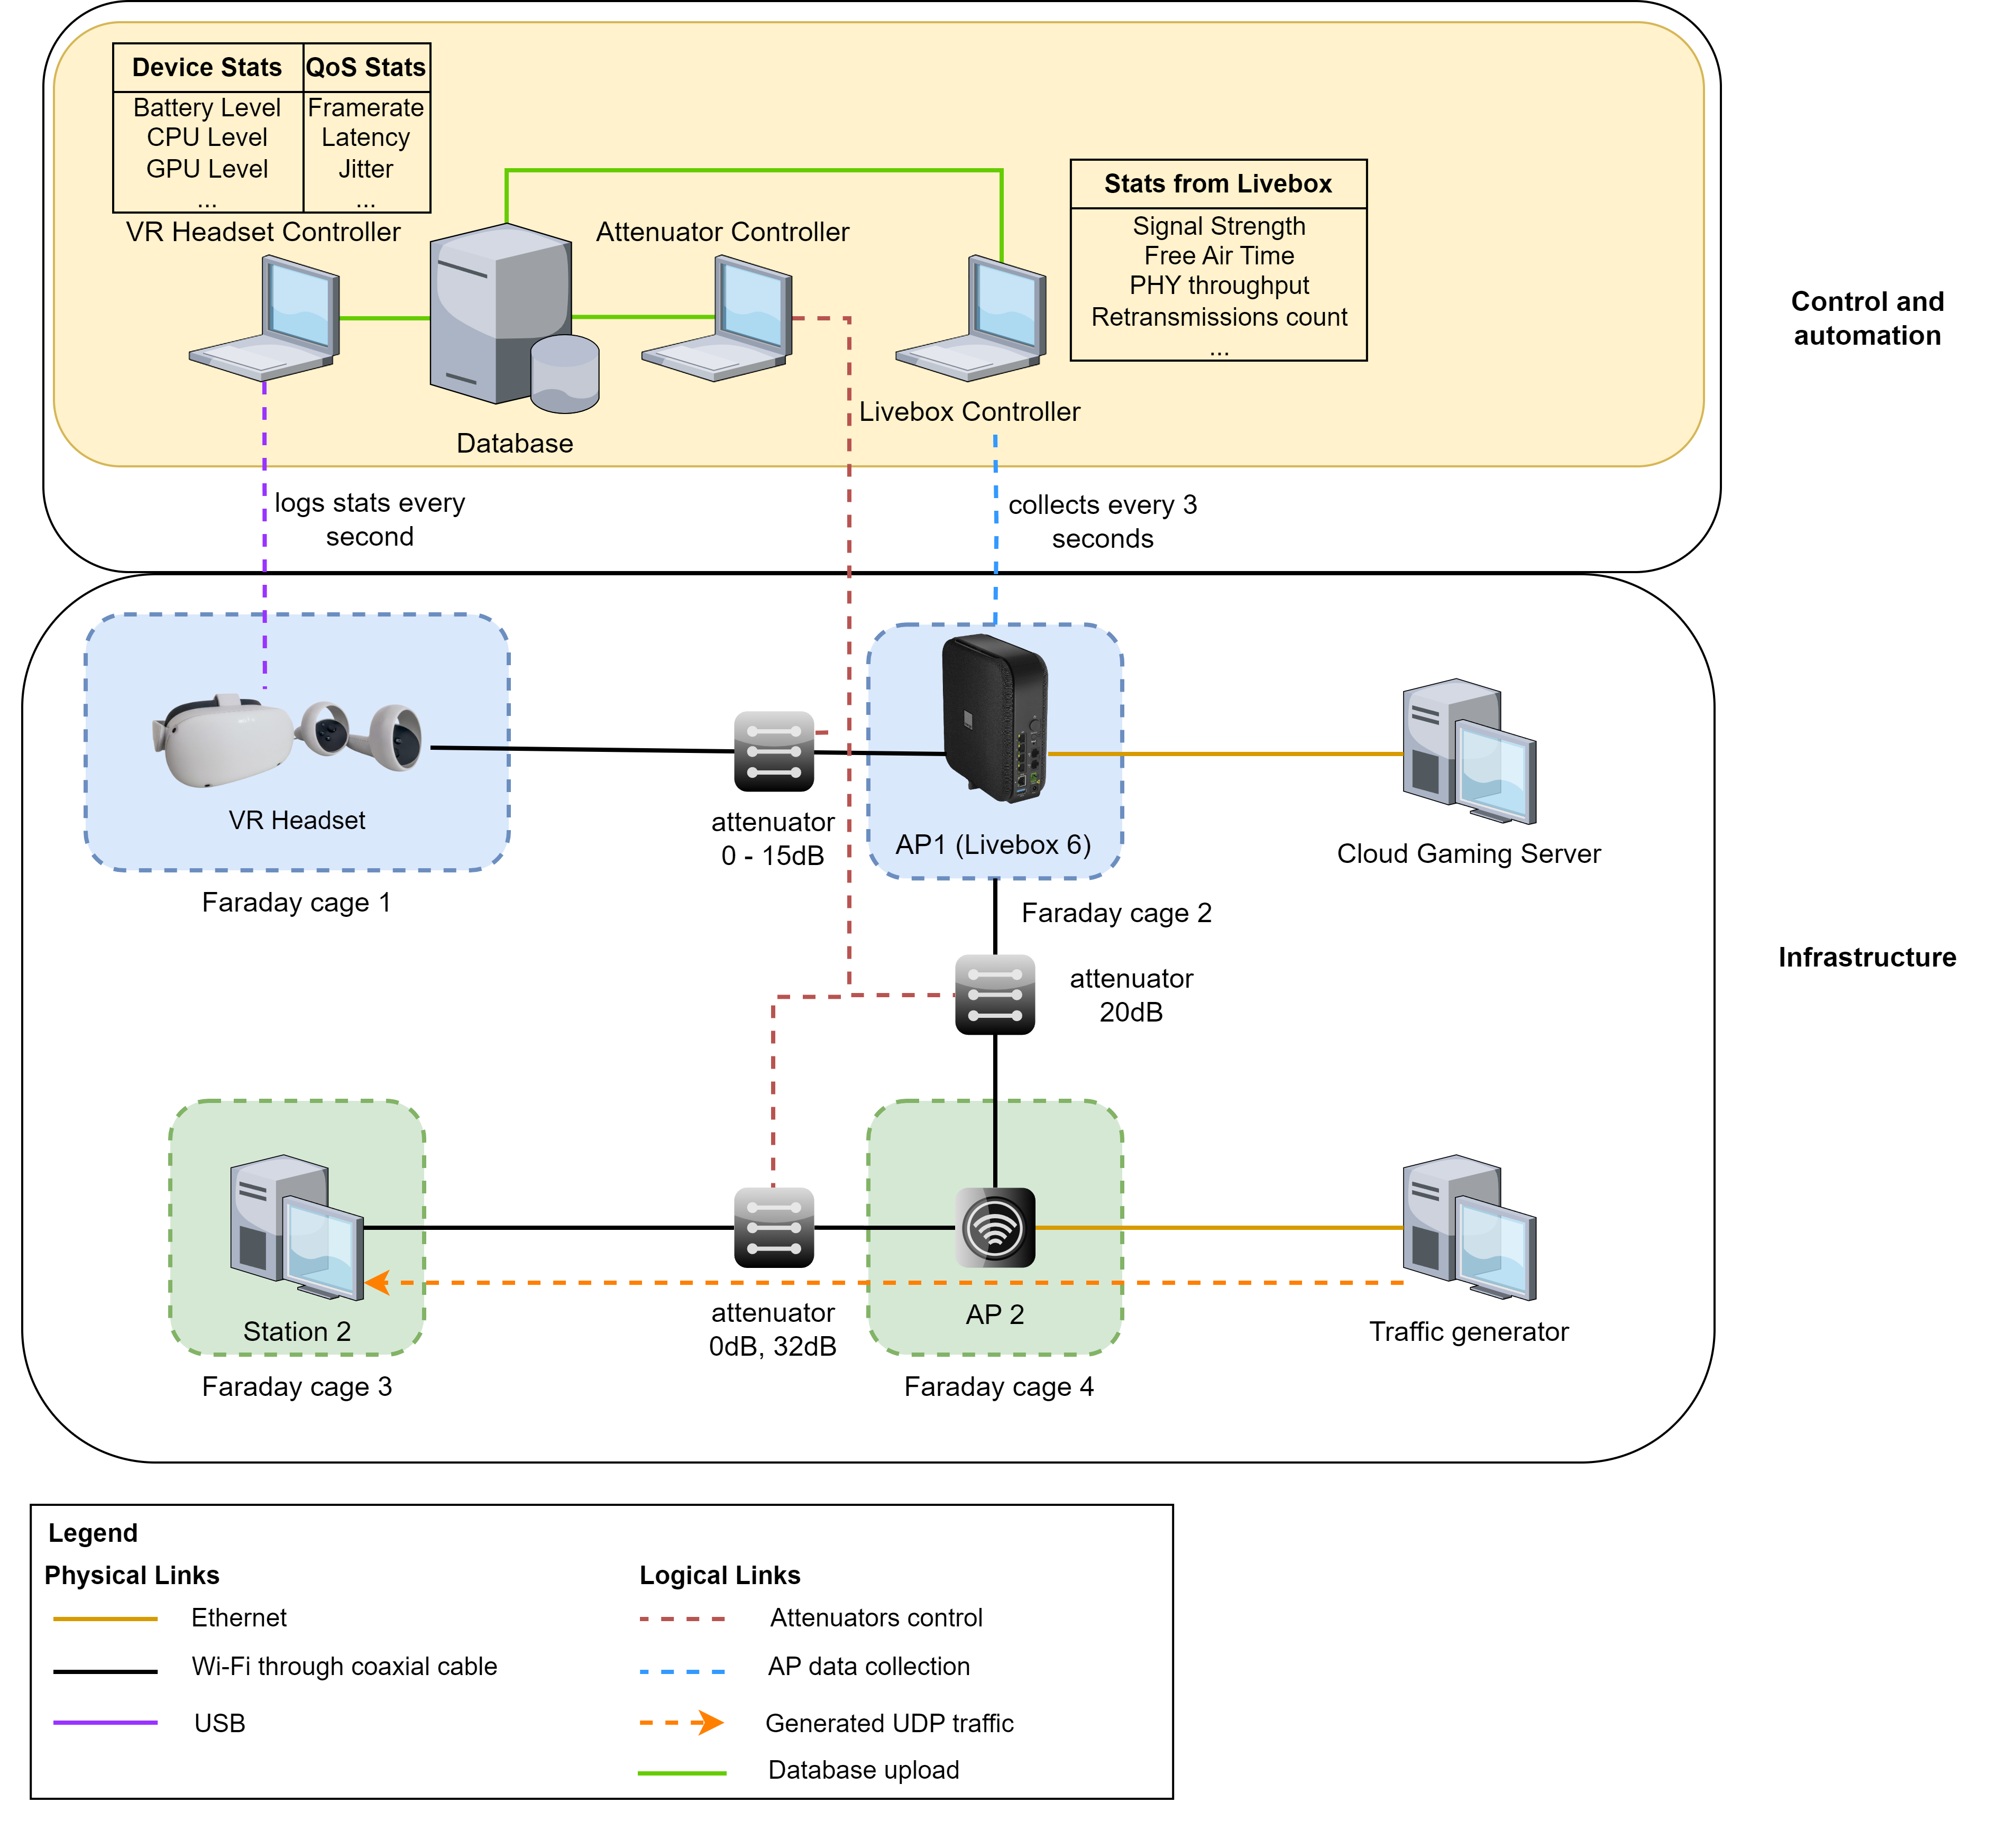
\includegraphics[width=\linewidth]{imgs/chapter_6/WiFi_testbed.png}
    \caption{Wi-Fi testbed for Cloud VR scenarios}
    \label{fig:chap_6:testbed_wifi}
\end{figure*}




\subsection{Wi-Fi Testbed for Controlled Experiments}

We designed a controlled Wi-Fi testbed, illustrated in Fig. \ref{fig:chap_6:testbed_wifi}, to replicate real-world Wi-Fi network impairments that can impact Cloud VR performance, with the goal of detecting these issues through root cause diagnosis.

The testbed consists of two primary layers:
\begin{itemize}
    \item \textbf{Infrastructure layer:} This layer includes up to four Faraday cages used to isolate equipment from external electromagnetic interference. The cages are allocated as follows: one for the VR headset, two for the APs, and one for a station used in interference scenarios. The layer also includes two access points (AP1 and AP2): AP1 is utilized for normal and coverage experiments, while AP2 introduces interference in specific scenarios. The Faraday cages are interconnected using coaxial cables to transmit Wi-Fi signals, and \ac{RF} attenuators \footnote{\url{https://adauratech.com/attenuators/}} are employed to simulate variations in signal strength during experiments. Two servers are part of this setup: the first server (see Fig. \ref{fig:chap_6:testbed}) runs the CloudVR software and is connected to AP1 via Ethernet, while the second server acts as a traffic generator connected to AP2, simulating competing downlink traffic using UDP.

    \item \textbf{Control and Automation layer:} This layer includes a VR PC controller connected to the VR headset via USB, responsible for managing headset settings and collecting performance metrics, such as key performance indicators (KPIs) from OVR Metrics tools\footnote{\url{https://developers.meta.com/horizon/downloads/package/ovr-metrics-tool/}} or quality-of-service (QoS) statistics from CloudXR. The controller also automates game sessions using the Meta Quest Autodriver\footnote{\url{https://developers.meta.com/horizon/documentation/unity/ts-autodriver}}. Additionally, this layer features an attenuator controller that configures and manages RF attenuators via APIs, enabling automated signal attenuation adjustments through FastAPI \footnote{\url{https://fastapi.tiangolo.com/}}. Furthermore, the Livebox controller manages the Livebox via Telnet to collect Wi-Fi KPIs every 3 seconds. A local ELK Stack \footnote{\url{https://www.elastic.co/fr/elastic-stack}} database aggregates data from all controllers for post-experiment analysis.

\end{itemize}

\subsection{Experimental Scenarios}

We collect Cloud VR data across several controlled scenarios using the Beat Saber game as a benchmark. These scenarios were executed on both the 2.4 GHz and 5 GHz frequency bands, as detailed below:
\begin{itemize}
    \item Normal scenarios: CloudVR sessions are conducted under ideal conditions, with no network impairments. The VR headset is placed in an optimal coverage area and connected to AP1 for each frequency band. A total of five 300-second sessions were performed for each of the frequency bands.
    \item Coverage scenarios: To simulate variations in signal strength, RF attenuators are used to modify the \ac{RSSI} during VR sessions. The following RSSI values were tested for 2.4 GHz: \{-55 dB, -60 dB, -65 dB\} and for 5 GHz: \{-80 dB, -85 dB, -90 dB\}. Each RSSI configuration is tested in three sessions, each lasting 100 seconds.
    \item Interference scenarios: Interference is introduced by a neighboring station connected to AP2, which operated on the same frequency and bandwidth as AP1. The interference is simulated by limiting the transmission opportunities (txops) available on AP1 after starting the game. The following interference levels were tested for 2.4 GHz: 85\% and 90\% of txops are occupied by AP2 and for 5 GHz: 89\%, 90\%, and 91\% of txops are occupied by AP2. Each interference configuration is tested in three sessions, with each session lasting 100 seconds.
\end{itemize}


This testbed design ensures a highly controlled environment for conducting CloudVR experiments. By leveraging Faraday cages, we eliminate uncontrolled external radio interference. The deployment of local servers minimizes external network variability, and automation tools enable seamless execution of experiments with precise configuration and data collection.





\section{Proposed Method}\label{chap_6:methodology}
In this section, we present our approach to root cause diagnosis for Cloud VR applications as a time series classification problem. The dataset of $T$ multivariate time series KPIs is represented as $\mathcal{D}_{train} =  \{(w_1, y_1), (w_2, y_2) \ldots, (w_T, y_T)\}$ where $w_t \in \mathbb{R}^{p \times m}$ is a $p \times m$-dimensional vector corresponding to the KPIs values for time steps $t, t+1, \ldots, t+p-1$, and $y_t$ is a one-hot encoded label vector of size $K$. $\forall j \in [|1, K|]$, $j=1$ if $w_t$ belongs to class $j$ and $y_{t,j}$ 0 otherwise.

The task of root cause diagnosis is to learn a classification model $f_\theta$ on $\mathcal{D}_{train}$ that can assign the root cause $y_t$ for any newly observed time series $\tilde{w}_t$. To achieve this, we propose RAID, a two-stage architecture comprising i) an \textbf{anomaly detection stage} and ii) a \textbf{root cause classification stage}.


\subsection{Anomaly detection stage}
The anomaly detection stage identifies whether a time series is anomalous, using a self-supervised learning approach based on contrastive learning. This stage eliminates the need for labeled data by leveraging only normal data collected during Cloud VR sessions without Wi-Fi impairments.
%$\mathcal{D}_{normal} =\{w_1, \ldots, w_N\}$ 
Traditional anomaly detection methods rely on techniques such as reconstruction-based, isolation-based, one-class classification, or generative models, which detect anomalies by modeling the concept of normality and measuring deviations from it. While effective, these approaches often fail to capture nuanced temporal dependencies and complex patterns in time-series data. 

\begin{figure*}[!ht]
    \centering
    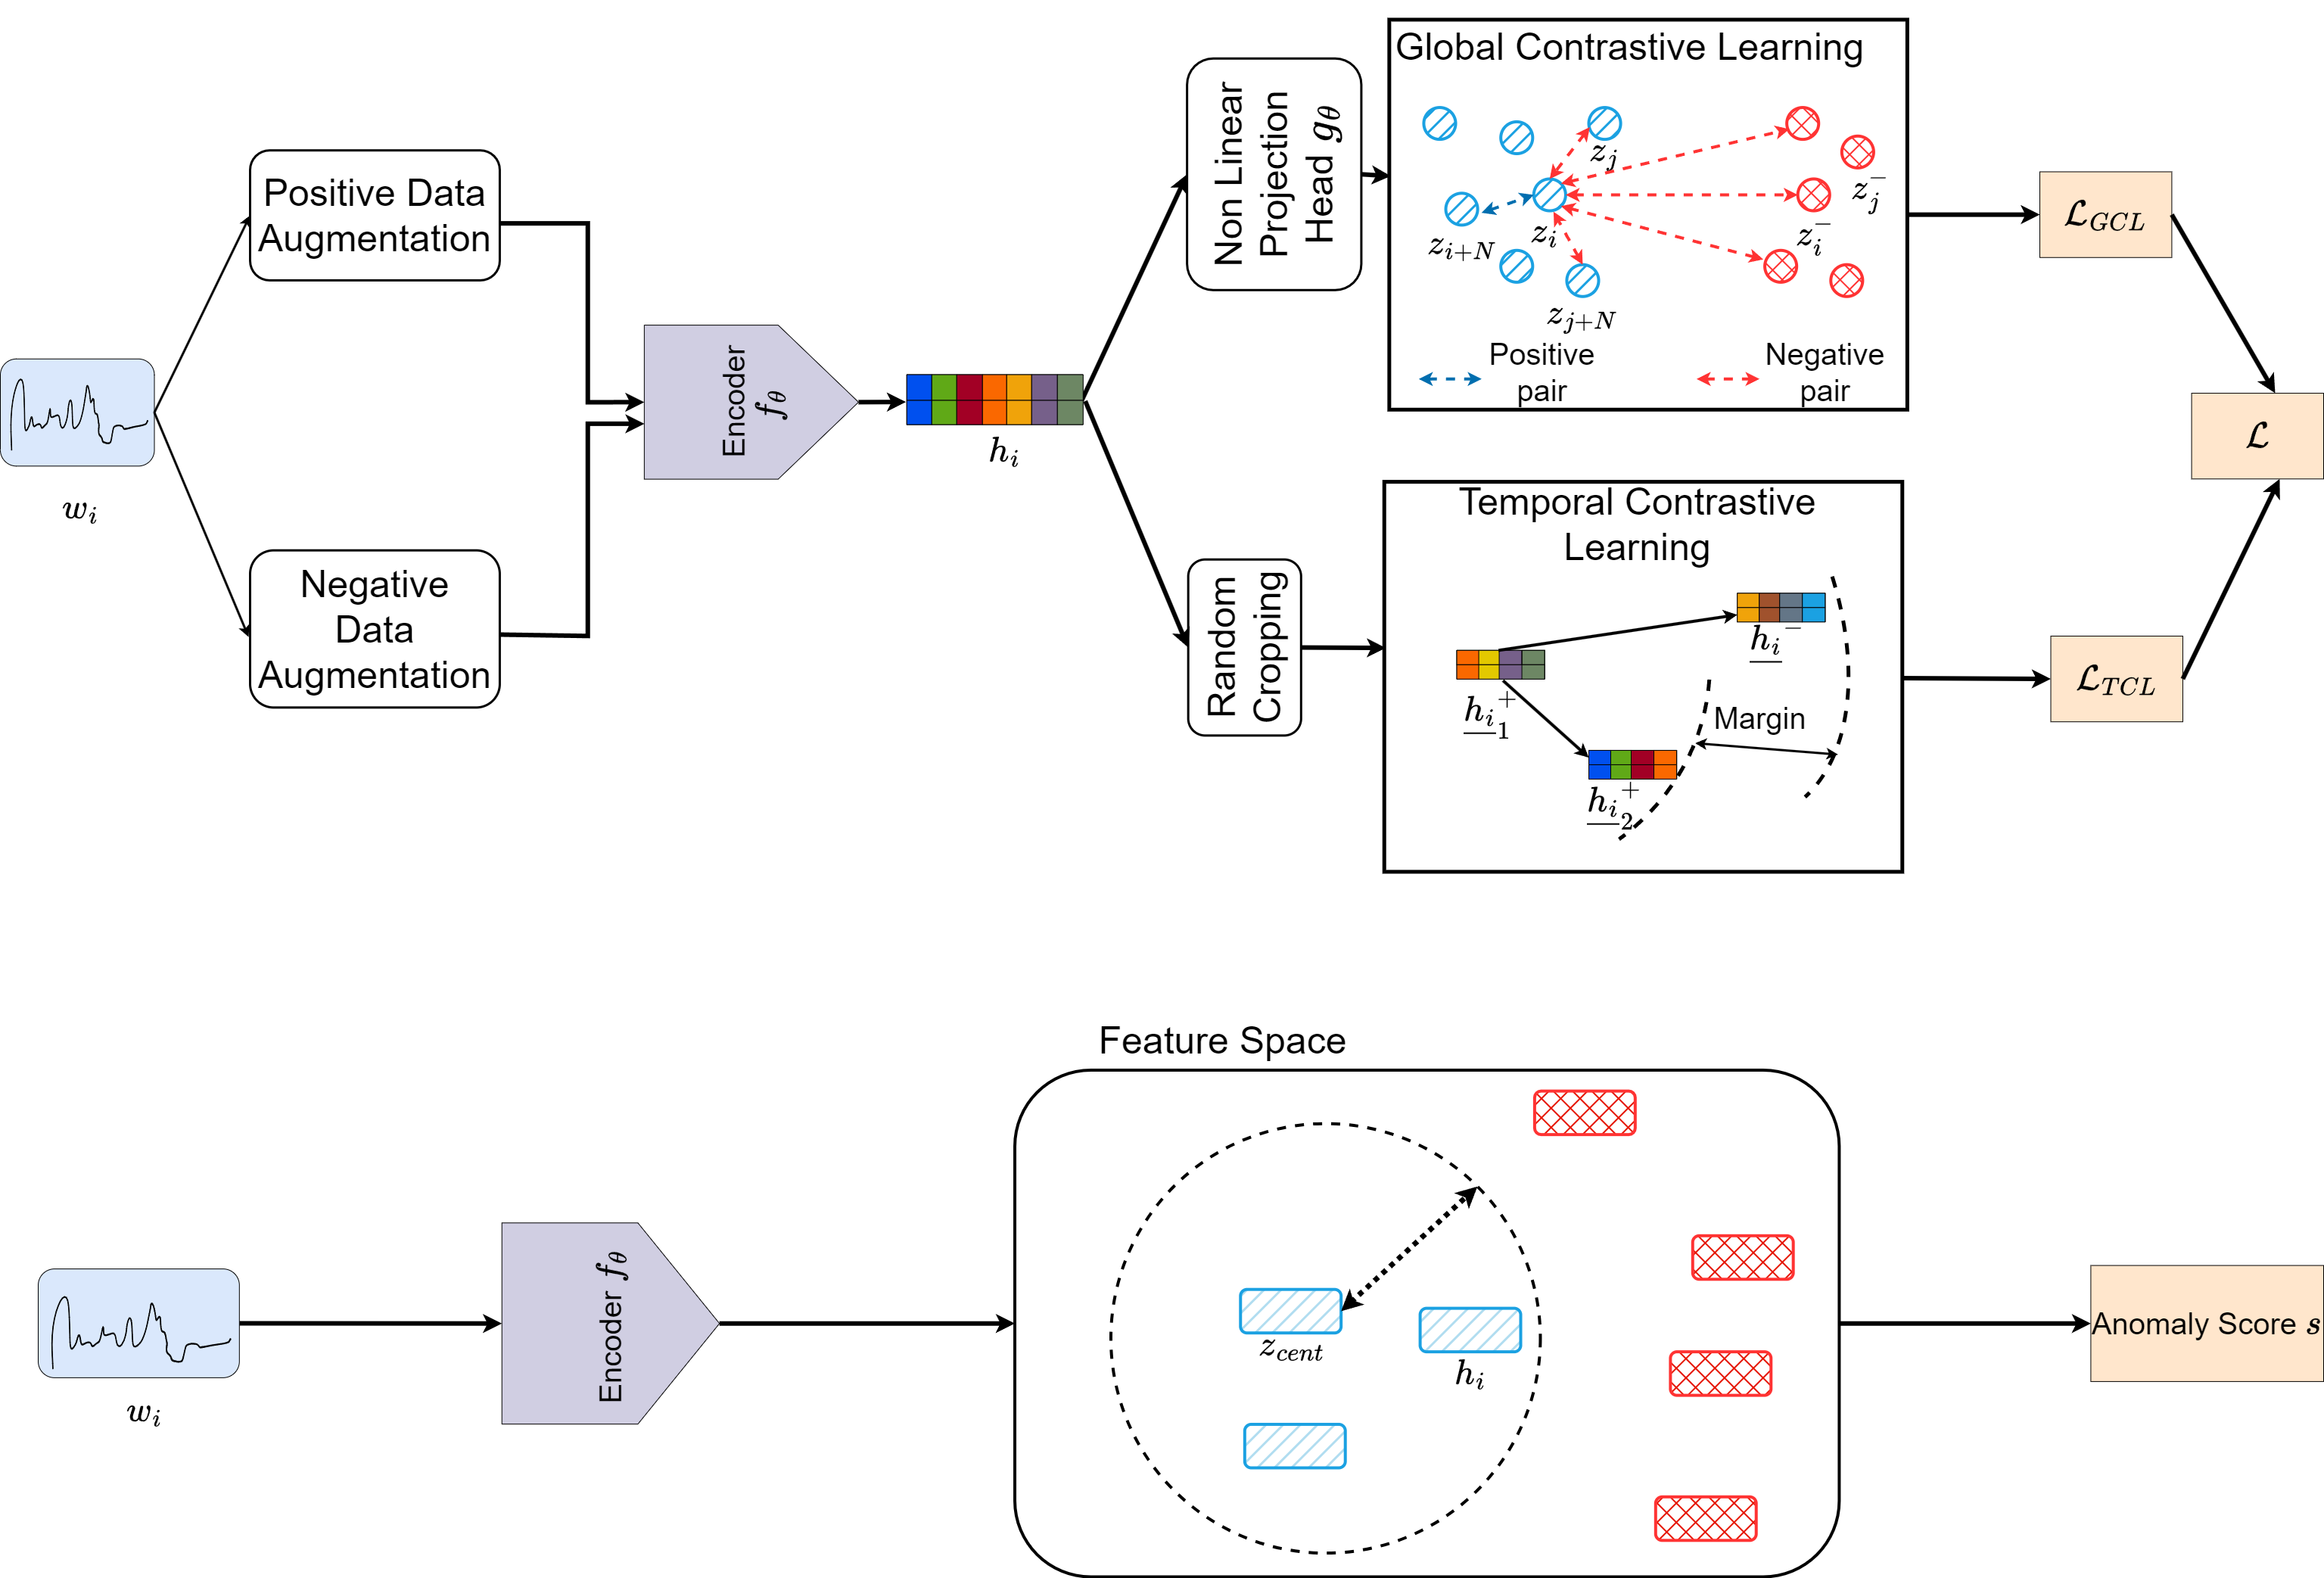
\includegraphics[width=\linewidth]{imgs/chapter_6/cats.png}
    \caption{Anomaly detector}
    \label{fig:chap_6:cats}
\end{figure*}

We adopt the CATS framework, summarized in Fig. \ref{fig:chap_6:cats}, described in Chapter \ref{chap:cats} which leverages temporal contrastive learning to learn robust representations of normal behavior. CATS enhances anomaly detection through synthetic anomaly generation and temporal contrastive loss formulations. The anomaly detector is trained using the loss combining global and temporal contrastive loss ($\frac{1}{2} (\mathcal{L}_{TCL} + \mathcal{L}_{GCL})$) and consists of the following components:
\begin{itemize}
    \item Data augmentation module. We generate views from time series: positive views using \textit{jitter} and \textit{scaling} to generate altered versions of normal data ensuring transformation-invariant representations. Synthetic anomalies are also generated using masking and trend transformations, bringing anomaly-related knowledge into the model.
    
    \item An encoder that encodes augmented time series into a low-dimensional latent space. The encoder is model-agnostic, allowing flexibility in its architecture (e.g., convolutional, recurrent, or transformer-based models).
    
    \item A projection head that maps the latent representations to a space optimized for contrastive learning. Typically implemented as a non-linear three-layer MLP \cite{chen2020simple}
    
    \item A temporal contrastive loss captures temporal similarity using a differentiable variant of DTW, Soft Dynamic Time Warping (Soft-DTW)-based triplet loss. This loss ensures that temporally similar representations are clustered while separating non-similar instances. This loss is defined as follows:
    \begin{equation}
        \mathcal{L}_{TCL} = \frac{1}{N} \sum_{i=1}^{N} max(D^{\gamma}(\underline{h_i}_1^+ - \underline{h_i}_2^+) - D^{\gamma}(\underline{h_i}_1^+ - \underline{h_i}^-) + m; 0)
    \end{equation}
    where $D^{\gamma}(.)$ is the Soft-DTW divergence measure, $m$ the margin parameter (minimum distance that must be kept between positive samples and negative samples).
    
    \item A global contrastive loss uses the Normalized Temperature-Scaled Cross-Entropy Loss (NT-Xent) to learn global feature similarities. This loss incorporates an expanded set of negative pairs to improve contrastive learning. \cite{chen2020simple}. This loss is defined as follows:
    \begin{equation}
        \mathcal{L}_{GCL} = \frac{1}{2N} \sum_{i \in \mathcal{B}^{+}} log \frac{exp(sim(z_i, z_{i+N})/\tau)}{\sum_{j \in \mathcal{B} \text{ and } j \neq i} exp(sim(z_i, z_j)/\tau)}
    \end{equation}
    with $\mathcal{B} = \mathcal{B}^{+} \cup \mathcal{B}^{-}$, $N$ the batch size, $\tau$ the temperature hyperparameter and $sim(.)$ the cosine similarity.
    
    \item Anomaly detection: After training, the encoder is retained to compute anomaly scores for unseen data. The score is the distance between the latent representation of the time series and the centroid of normal representations. An anomaly is flagged if the score exceeds a predefined threshold. The anomaly score is defined as follows:
    \begin{equation}
    \begin{split}
        s(\tilde{w_t}) &= \mathcal{D}(f_{\theta}(\tilde{w_t}), z_{cent}) \\
                       &=  \mathcal{D}(\tilde{z_t}, z_{cent}) \\
                       &=  \mathcal{D}(\tilde{z_t}, \frac{1}{N_{train}} \sum_{i=1}^{N_{train}} w_i) \\
    \end{split}
    \end{equation}
    where $\mathcal{D}$ is the Euclidean distance.
\end{itemize}

% \subsection{Root cause classification}
% Once an anomaly is detected, the next step is to determine its underlying root cause. This stage is framed as a supervised classification problem, where the objective is to map each detected anomaly to a predefined class of root causes $\{cause_1, cause_2, \ldots, cause_{K-1}\}$. To ensure efficiency and simplicity, we use a shallow classifier such as logistic Regression or Support Vector Machine (SVM) despite the various techniques for supervised TSC that were proposed in the literature. This approach, as showed in the following sections, achieves high accuracy with minimal computational overhead, making it suitable for real-time deployment.

\subsection{Root Cause Classification}

Once an anomaly is detected, the next step is to determine its underlying root cause. This stage is framed as a supervised classification problem, where the objective is to map each detected anomaly to a predefined class of root causes $\{cause_1, cause_2, \ldots, cause_{K-1}\}$.

To ensure efficiency and simplicity, we use a shallow classifier, a \ac{SVM}. Despite the numerous techniques for supervised TSC proposed in the literature, this model is efficient enough for our task given the anomaly detection stage previously executed. 

SVM are supervised learning algorithms designed to find the optimal hyperplane that separates data into distinct classes in a feature space. In the context of root cause classification, the input of time series flagged as anomalies ${(x_i, y_i)}_{i=1}^{N_{train}}$ are fed as input to the SVM classifier. The SVM employs a kernel trick (a kernel function $k$ satisfying $k(x_i, x_j) = \phi(x_i) \phi(x_j)$) to map inputs into a higher-dimensional space where a linear separation is possible. We use the \ac{RBF} kernel function ( $k(x_i, x_j) = \exp(-\gamma |x_i - x_j|^2)$). The classifier next identifies the hyperplane that maximizes the margin between the classes by solving the dual problem.

\begin{equation}
\begin{split}
    \min_{\alpha} & \quad \frac{1}{2} \sum_{i, j=1}^{N_{train}} \alpha_i \alpha_j y_i y_j k(x_i, x_j) - \sum_{i=1}^{N_{train}}  \alpha_i, \\
    \text{s.t} \quad & 0 \leq \alpha_i \leq C, \quad \forall i = 1, \ldots, N_{train} \\
                & \sum_{i=1}^{N_{train}}  \alpha_i y_i = 0
\end{split}
\end{equation}


where $\alpha_i$ are the Lagrange multipliers obtained by solving the dual optimization problem; $C > 0$ is the regularization parameter that controls the trade-off between maximizing the margin and minimizing classification errors; $y_i$ are the labels of the training data points and $x_i$ are the feature vectors of the training data.
% \begin{itemize}
%     % \item $w$ is the weight vector defining the orientation of the hyperplane.
%     % \item $b$ is the bias term determining the offset of the hyperplane from origin.
%     %\item $K(\mathbf{x}_i, \mathbf{x}_j)$ is the kernel function, defined as $K(\mathbf{x}_i, \mathbf{x}_j) = \phi(\mathbf{x}_i)^\top \phi(\mathbf{x}_j)$, which computes the dot product in the feature space induced by $\phi$.
%     \item $\alpha_i$ are the Lagrange multipliers obtained by solving the dual optimization problem.
%     \item $C > 0$ is the regularization parameter that controls the trade-off between maximizing the margin and minimizing classification errors.
%     \item $y_i$ are the labels of the training data points.
%     \item $x_i$ are the feature vectors of the training data.
% \end{itemize}

Each input $\tilde{x}$ is then assigned to one of the predefined cause $\tilde{y}$ as follows:

\begin{equation}
    \tilde{y} = \text{sign}(\sum_{i=1}^{N_{train}} \alpha_i y_i K(x_i, \tilde{x}) + b),
\end{equation}

For multi-class classification with $K > 2$, SVM is extended using one-vs-one strategies where $\frac{K(K-1)}{2}$ binary classifiers are trained, each distinguishing between two classes and the class with the highest votes is chosen. 


\begin{figure*}[!ht]
    \centering
    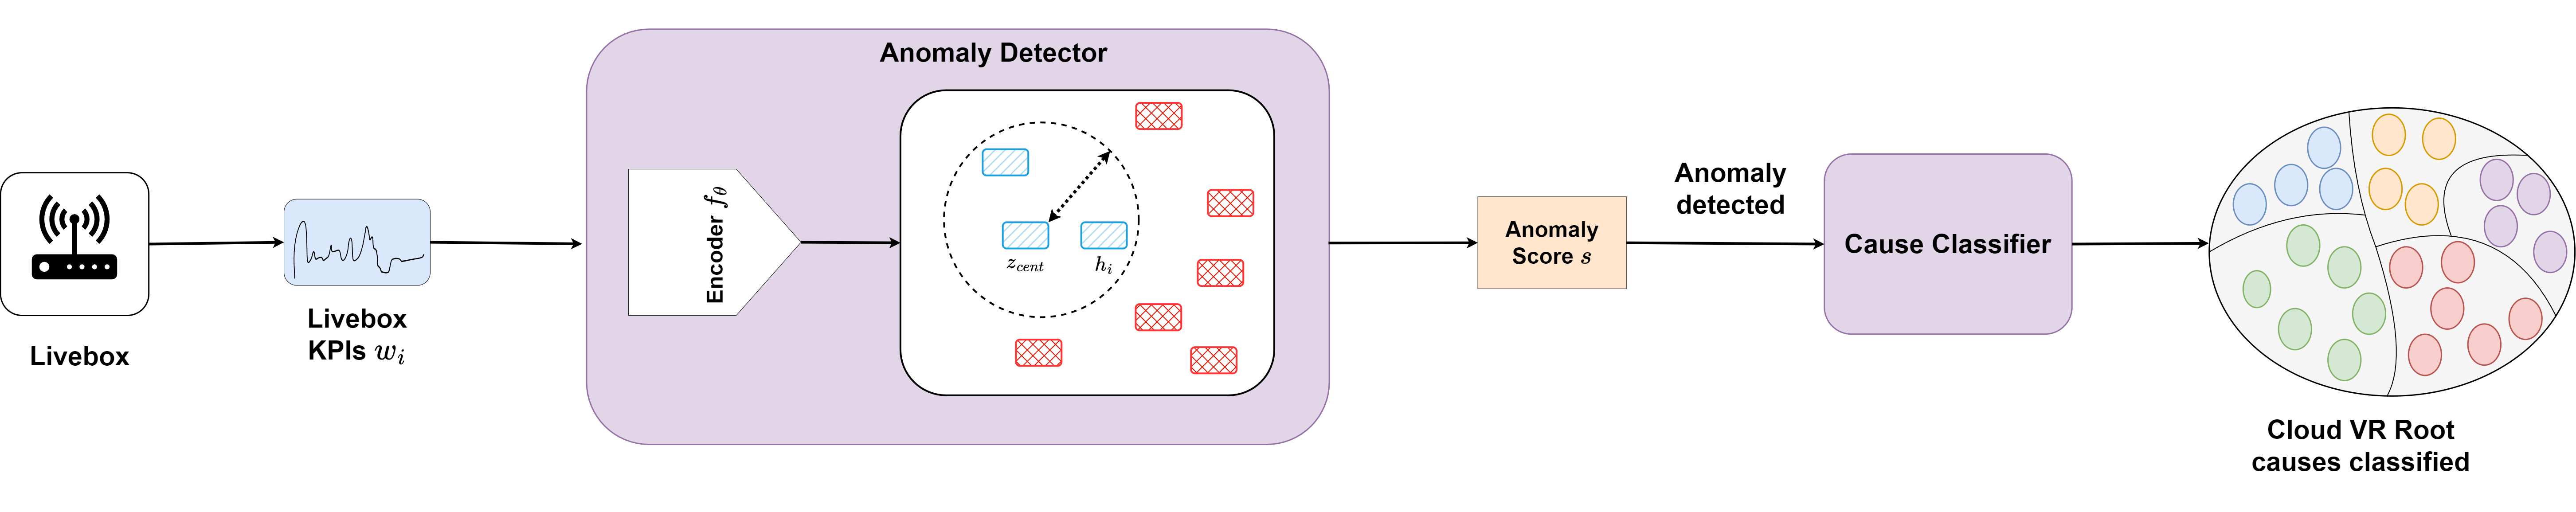
\includegraphics[width=\linewidth]{imgs/chapter_6/diagnostic_rcd.png}
    \caption{RAID framework}
    \label{fig:chap_6:raid}
\end{figure*}

% The rationale behind this choice is motivated by SSL-based classification setups: after learning representations using SSL, the encoder have can discriminate different class so that a shallow classifier trained on top of the representation is sufficient to make predictions.

% The CATS framework's encoder learns discriminative representations that make it easier for a simple classifier to achieve high accuracy. This choice aligns with the principle of leveraging self-supervised representations for downstream supervised tasks.


% \subsection*{Pseudocode for Our Solution}

% \begin{lstlisting}[caption={Anomaly Detection and Root Cause Diagnosis}, label={lst:solution}]
% def train_CATS_model(window_time_series):
%     # Data Augmentation
%     pos_view_1, pos_view_2, neg_view = data_augmentation(window_time_series)
    
%     # Encoding
%     h_pos_1 = encoding(pos_view_1)
%     h_pos_2 = encoding(pos_view_1)
%     h_neg = encoding(pos_view_1)
    
%     # Projection head
%     z_pos_1 = projection(h_pos_1)
%     z_pos_2 = projection(h_pos_2)
%     z_neg = projection(h_neg)
    
%     # Compute the loss function
%     l_gcl = gcl_loss(z_pos_1, z_pos_2, z_neg)
%     l_tcl = tcl_loss(h_pos_1, h_pos_2, h_neg)
    
%     l_total = (l_gcl + l_tcl) / 2
    
%     # Backpropagate
%     l_total.backward()

% def anomaly_detection(data, anomaly_threshold):
%     # Data processing
%     features = preprocess(data)
    
%     # Compute the anomaly score
%     anomaly_score = anomaly_detector(features)
    
%     # Check if the data is anomaly or not
%     if (anomaly_score <= threshold):
%         return normal
%     else: # Anomalies detected => Apply the classifier
%         pred = cause_classifier(features)
%         return pred
    
% \end{lstlisting}



\section{Evaluation setup}\label{chap_6:evaluation}
\subsection{Dataset Description}

To evaluate our proposed solution, we utilize the time series datasets collected from the experimental testbed described in Chapter \ref{chap:measurements}. Although our setup gathers KPIs from both the VR headset and the CloudXR stack, which provide insights into QoS and QoE during VR sessions, this study focuses exclusively on data retrieved from the Livebox. This choice is motivated by the practical accessibility of these metrics for network operators, who own and manage the Livebox. Leveraging these metrics for RCD allows for the development of smarter APs and more intelligent network management solutions, aligning closely with the operational needs of network operators.

The dataset consists of 112 time series features extracted from the Livebox. These features include signal strength indicators (e.g., RSRP, RSSI), transmission performance metrics (e.g., txops), channel utilization measures (e.g., air time), among others, offering a comprehensive view of Wi-Fi performance in various conditions. Monitoring was performed at a frequency of one sample every three seconds. To facilitate analysis, the data is structured into overlapping time series windows, each spanning 10 time steps (30 seconds per window). 

In total, the dataset contains 13,657 time series windows, which are partitioned into training and testing subsets using a 70:30 split ratio. The training set contains 9,524 windows, while the test set consists of 4,133 windows. The dataset is further categorized into three classes, corresponding to distinct experimental scenarios during data collection:


A summary of the dataset, including the class-wise breakdown of training and test samples, is presented in Table \ref{tab:chap_6:datasets}.

\begin{table}[ht]
\begin{threeparttable}
\caption{Dataset Summary}
\label{tab:chap_6:datasets}
\setlength\tabcolsep{0pt} % make LaTeX figure out intercolumn spacing

\begin{tabular*}{\columnwidth}{@{\extracolsep{\fill}} l c c c c }
\toprule

\bf Class & \bf Train Size & \bf Test Size & \bf Number of Features & \bf Number of Time Steps \\
\midrule
\bf Normal & 4718 & 1924 & 112 & 10 \\
\bf Attenuation & 2984 & 1270 & 112 & 10 \\
\bf Interference & 1822 & 939 & 112 & 10 \\
\midrule
\bf Overall & 9524 & 4133 & 112 & 10 \\
\bottomrule
\end{tabular*}
\end{threeparttable}
\end{table}

%The well-balanced representation of classes in the dataset supports robust evaluation of the proposed model. Furthermore, the high temporal resolution of the features ensures that our solution can capture subtle temporal patterns critical for accurately distinguishing between the classes.

\subsection{Competing Solutions}
To demonstrate the effectiveness of our proposed solution, we compare it against several baselines. These include both one-stage and two-stage time series classification (TSC) models. 

\subsubsection{One-Stage Models}
For the one-stage models, we include the following:
\begin{itemize}
    \item \textbf{1-NN-DTW:} The nearest neighbor classifier paired with a distance function. When combined with Dynamic Time Warping (DTW) as the distance measure, this model has proven to be a strong baseline for time series classification across numerous benchmarks \cite{bagnall2017great}. 
\end{itemize}

We also evaluate self-supervised time series representation learning methods, which have demonstrated efficiency in TSC. Following the protocol outlined in \cite{franceschi2019unsupervised}, these models undergo an unsupervised pre-training stage, after which an SVM classifier with an RBF kernel is trained on the learned representations for downstream classification. The selected methods are:
\begin{itemize}
    \item \textbf{T-Loss \cite{franceschi2019unsupervised}:} A self-supervised learning approach that uses a novel triplet loss with time-based negative sampling to obtain representations general enough for downstream tasks, even when dealing with variable-length, multivariate time series.
    \item \textbf{TS-TCC \cite{Eldele2021TimeSeriesRL}:} A self-supervised framework for time series representation learning that employs weak and strong time series augmentations to create different views. These views are used in temporal and contextual contrastive modules to learn robust and discriminative representations.
    \item \textbf{TS2Vec \cite{Yue2021TS2VecTU}:} A framework designed to learn both instance-wise and temporal-wise information for robust time series representations. It utilizes a hierarchical contrastive objective applied to augmented views of time series, achieving excellent results in TSC tasks.
\end{itemize}

\subsubsection{Two-Stage Models}
For the two-stage models, we replace the CATS model in the first stage with unsupervised anomaly detection methods. The selected models are:
\begin{itemize}
    \item \textbf{iForest \cite{liu2008isolation}:} An isolation-based unsupervised anomaly detection model. It isolates anomalies by recursively performing random splits on the feature values. Anomalous samples are easier to isolate due to their significant deviation from the normal data, requiring fewer splits.
    \item \textbf{USAD \cite{audibert2020usad}:} UnSupervised Anomaly Detection is a deep learning-based approach employing two autoencoders in a min-max game. The first autoencoder learns to reconstruct input data, while the second attempts to differentiate between true data and reconstructions.
    \item \textbf{SimCLR \cite{chen2020simple}:} A contrastive learning framework originally proposed for computer vision and adapted for time series. It learns representations from augmented views of data and can be used for anomaly detection following a procedure similar to the CATS framework.
\end{itemize}

\subsection{Evaluation Metrics}
We evaluate the performance of our root-cause diagnosis models using well-known multi-class classification metrics, including weighted Precision (P), weighted Recall (R), weighted F1-score (F1), Accuracy (Acc), and Normalized Accuracy (N-Acc). These metrics are defined as follows:
\begin{itemize}
    \item \textbf{Precision:} The macro-weighted precision is the weighted average of precision values computed for each class, $w_i$ being the proportion of class $i$:
        \begin{equation}
            P = \sum_{i=1}^{K} w_i \times P_i, \quad P_i = \frac{TP_i}{TP_i + FP_i}
        \end{equation}
    \item \textbf{Recall:} The macro-weighted recall is the weighted average of recall values computed for each class, $w_i$ being the proportion of class $i$:
        \begin{equation}
            R = \sum_{i=1}^{K} w_i \times R_i, \quad R_i = \frac{TP_i}{TP_i + FN_i}
        \end{equation}
    \item \textbf{F1-Score:} The macro-weighted F1-score is the harmonic mean of macro-weighted Precision and Recall. This metric coupled P and R are suitable for imbalanced datasets.
        \begin{equation}
            F1 = 2 \times \frac{P \times R}{P + R}
        \end{equation}
    \item \textbf{Accuracy:} The fraction of correctly classified samples over the total number of samples. This metric is widely used and easy to interpret.
    \item \textbf{Normalized Accuracy (N-Acc):} This metric adjusts the balanced accuracy ($bac = \frac{1}{K} \sum_{i=1}^{K} w_i \times R_i$)  which is the weighted average of the recall of each class with respect to the accuracy of random guessing ($bac_{RG}$), ensuring that random predictions score 0 while perfect predictions score 1. It is more interpretable and suitable for imbalanced datasets.
        \begin{equation}
            \text{N-Acc} = \frac{bac - bac_{RG}}{1 - bac_{RG}}
        \end{equation}
\end{itemize}

\subsection{Implementation details}
The datasets collected are normalized and splits into training and test sets.
For our detector solution, we use the same implementation details as CATS architecture. This consists in a dilated CNN module with ten residual blocks of 1D convolutional layers as encoder; a three-layer MLP with ReLU activation as projection head. The data augmentation techniques include \textit{jitter}, \textit{scaling} for positive views and \textit{masking} and \textit{trend} for negative views. The anomaly detection framework is trained with temporal and global contrastive loss optimized using the Adam optimizer with a learning rate of $10^{-3}$, the batch size is 512 and training is conducted for 100 epochs. The

For competing solutions, we rely on publicly available implementations provided on Github. We use the same epochs, optimizer, learning rate and batch size. After pretraining of SSL competing solutions, classification is performed using a SVM with an RBF kernel. Hyper-parameters of the SVM are fine-tuned using a grid search procedure to achieve optimal performance.

Experiments are performed on a Ubuntu 22.04 with AMD Ryzen 9 5900X 12-Core Processor and a NVIDIA RTX 3090 Ti of 24GB. Python 3.10.12 is used as programming language, PyTorch 2.2.0 as the deep learning framework and CUDA 12.1 for GPU acceleration. The code and datasets to reproduce all the experiments are provided. All details, implementation and hyper-parameters are included.


\section{Results}\label{chap_6:results}
\subsection{Performance Evaluation}

Table \ref{tab:chap_6:benchmark} summarizes the evaluation results of our solution compared to competing TSC methods using various performance metrics, including accuracy, normalized accuracy, precision, recall, and F1-score. The results highlight the superiority of our approach over both one-stage and two-stage methods.


\begin{table*}[t]
\caption{Performance comparison on the datasets. Mean and standard deviation computed over five runs for Cloud VR datasets. Bold values indicate best results and underlined values the second best.}

\label{tab:chap_6:benchmark}
\setlength\tabcolsep{2pt}
\begin{tabular*}{\textwidth}{@{\extracolsep{\fill}}l | l | ccccc }
\toprule
\bf Models & \bf Metrics & \bf Accuracy & \bf N-Accuracy & \bf Precison & \bf Recall & \bf F1-score \\
\midrule
\multirow{4}{*}{\rotatebox{90}{\bf One-stage}} & 1-NN-DTW & 51.54$_{(\pm0.11)}$ & 26.36$_{(\pm0.17)}$ & 56.74$_{(\pm0.09)}$ & 51.54$_{(\pm0.11)}$ & 52.96$_{(\pm0.10)}$ \\
%& NN-DTW & $_{(\pm)}$ & $_{(\pm)}$ & $_{(\pm)}$ & $_{(\pm)}$ & $_{(\pm)}$ \\
\addlinespace
\cmidrule{2-7}
& T-Loss & \underline{79.47$_{(\pm4.39)}$} & \bf 75.22$_{(\bf\pm5.58)}$ & \bf 83.98$_{(\bf\pm4.74)}$ & \underline{79.47$_{(\pm4.39)}$} & \underline{79.60$_{(\pm4.53)}$} \\
\addlinespace
& TS2Vec & 70.12$_{(\pm5.28)}$ & 55.71$_{(\pm6.53)}$ & 75.42$_{(\pm3.22)}$ & 70.12$_{(\pm5.28)}$ & 70.49$_{(\pm4.88)}$ \\
\addlinespace
& TS-TCC & 73.78$_{(\pm6.38)}$ & 66.17$_{(\pm8.12)}$ & 79.29$_{(\pm6.07)}$ & 73.78$_{(\pm6.38)}$ & 73.86$_{(\pm6.68)}$ \\
\addlinespace
%& NN-DTW & $_{(\pm)}$ & $_{(\pm)}$ & $_{(\pm)}$ & $_{(\pm)}$ & $_{(\pm)}$ \\

\addlinespace
\midrule

\multirow{4}{*}{\rotatebox{90}{\bf Two-stage}} & iForest & 72.48$_{(\pm2.69)}$ & 62.22$_{(\pm4.69)}$ & 72.26$_{(\pm3.14)}$ & 72.48$_{(\pm2.69)}$ & 72.24$_{(\pm2.99)}$ \\
\addlinespace
& USAD & 72.22$_{(\pm0.80)}$ & 63.39$_{(\pm1.36)}$ & 72.72$_{(\pm0.97)}$ & 72.22$_{(\pm0.80)}$ & 72.38$_{(\pm0.84)}$ \\
\addlinespace
& SimCLR & 57.76$_{(\pm3.25)}$ & 37.59$_{(\pm4.84)}$ & 61.01$_{(\pm2.60)}$ & 57.76$_{(\pm3.25)}$ & 58.65$_{(\pm3.06)}$ \\
\addlinespace
\cmidrule{2-7}
\rowcolor{FireBrick!40}  & \bf RAID & \bf 81.83$_{(\bf \pm2.96)}$ & \underline{74.80$_{(\pm4.19)}$} & \underline{81.85$_{(\pm3.02)}$} & \bf 81.83$_{(\bf \pm2.96)}$ & \bf 81.60$_{(\bf \pm3.05)}$ \\
\addlinespace


\bottomrule
\end{tabular*}
\end{table*}
 % \rowcolor{FireBrick!40} 

\subsubsection{Evaluation of One-Stage Models}
One-stage models, including 1-NN-DTW, T-Loss, TS2Vec, and TS-TCC, directly perform root cause classification without a preliminary anomaly detection step. Among these models, 1-NN-DTW exhibits the lowest overall performance, with an accuracy of 51.54\% and an F1-score of 52.96\%. Despite being a strong baseline for TSC, it struggles to handle the complex time-series data encountered in CloudVR scenarios.

Contrastive learning-based SSL models outperform 1-NN-DTW. Among them, T-Loss emerges as the most effective technique, achieving the highest normalized accuracy (75.22\%) and precision (83.98\%) within this category. This demonstrates its capability to learn meaningful representations for RCD tasks. TS-TCC follows with an accuracy of 73.78\% and an F1-score of 73.86\%, while TS2Vec achieves an accuracy of 70.12\% and an F1-score of 70.49\%.

\subsubsection{Evaluation of Two-Stage Models}
Two-stage models incorporate a preliminary anomaly detection step, enabling better focus on relevant patterns before root cause classification. iForest and USAD achieve comparable performance, with accuracy scores of 72.48\% and 72.22\%, respectively. Both models demonstrate strong F1-scores around 72\%, yet they fall short of advanced one-stage approaches like T-Loss. Meanwhile, SimCLR performs suboptimally with an accuracy of 57.76\% and an F1-score of 58.65\%.

Our proposed solution significantly outperforms all competing methods across most metrics. It achieves the highest accuracy (81.83\%), recall (81.83\%), and F1-score (81.60\%), demonstrating robustness and effectiveness for CloudVR RCD. While T-Loss marginally outperforms in normalized accuracy and precision, our model achieves the best balance across all metrics, establishing it as the most reliable approach in this evaluation.

The superior performance of our solution can be attributed to the efficiency of its anomaly detection stage. As shown in Fig. \ref{fig:chap_6:ad_results}, our solution outperforms other two-stage techniques in detecting anomalies across various well-known metrics. RAID achieves the best overall anomaly detection performance, which directly contributes to its effectiveness in RCD tasks.


\begin{figure*}[!ht]
    \centering
    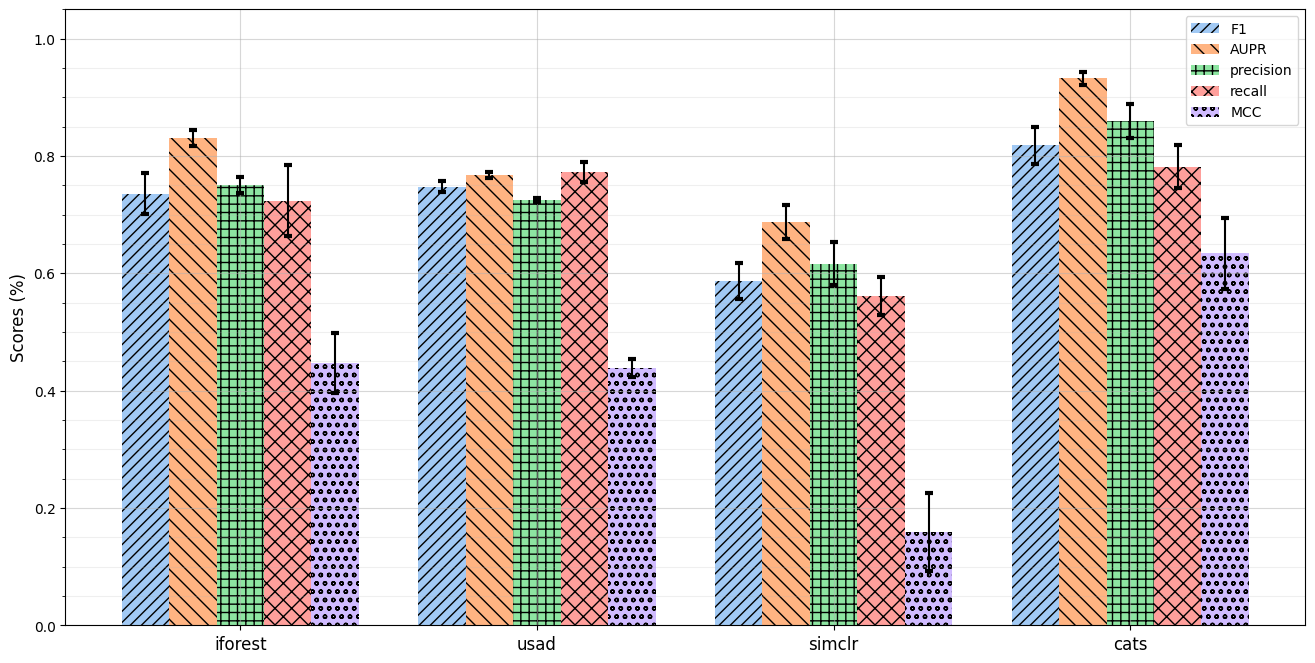
\includegraphics[width=.9\linewidth]{imgs/chapter_6/ad.png}
    \caption{Results of anomaly detectors of two-stage models.}
    \label{fig:chap_6:ad_results}
\end{figure*}


\subsubsection{Per-Class Performance Analysis}

Figures \ref{fig:chap_6:confusion_matrix} and \ref{fig:chap_6:per_class} provide a detailed comparison of the per-class performance metrics for T-Loss and RAID. Our approach demonstrates a significant advantage in efficiently distinguishing normal scenarios from both coverage and interference scenarios.

For normal scenarios, our solution achieves a notably lower misclassification rate compared to T-Loss, with 1,761 correctly classified normal samples versus 1,350 for T-Loss. This represents a substantial improvement in detecting normal behavior. Additionally, our solution attains perfect classification for interference scenarios, with a recall of 100\%, highlighting its robustness in detecting distinct anomaly patterns such as interference.

However, Fig. \ref{fig:chap_6:per_class} also reveals the limitations of our solution. It struggles to discriminate coverage scenarios, with a considerable number of coverage windows misclassified as normal. This indicates challenges in capturing the subtle variations and transitional patterns between normal and coverage states. In contrast, T-Loss, while less accurate overall, shows a more balanced performance in handling coverage scenarios. 

This trade-off underscores the strengths and weaknesses of our model: it is highly effective in detecting clear-cut anomalies but requires further refinement to enhance its sensitivity to nuanced variations between normal and coverage states. Future work could focus on addressing this limitation by incorporating advanced feature extraction techniques or domain-specific data augmentation strategies.


\takeaway{RAID model demonstrates superior performance in root cause diagnosis for Cloud VR scenarios, achieving the highest performance compared to both one-stage and two-stage approaches. Its robust anomaly detection stage significantly enhances its effectiveness, outperforming other methods in detecting distinct patterns such as interference. However, the model struggles with subtle variations in coverage scenarios, suggesting room for improvement in handling nuanced transitions.}

\begin{figure*}[!t]
  \centering
  \begin{tabular}{ c @{\hspace{0pt}} c}
  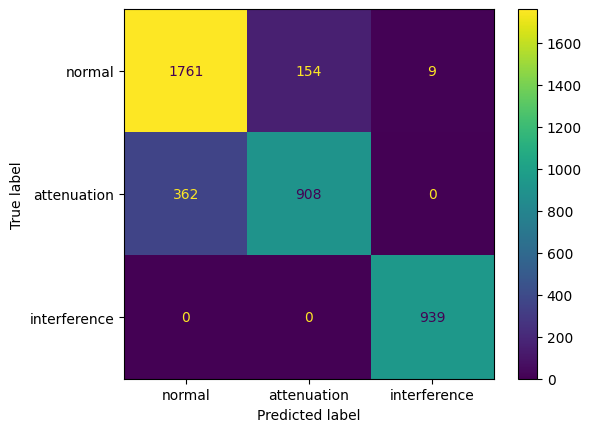
\includegraphics[width=0.5\textwidth]{imgs/chapter_6/cm_cats.png}
    &
  %\medskip
    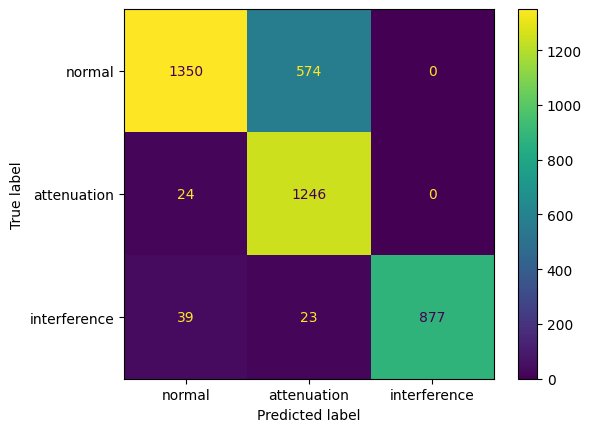
\includegraphics[width=0.5\textwidth]{imgs/chapter_6/cm_triplet.png}\\
     \small \textbf{(a) RAID} &
    \small \textbf{(b) T-Loss}  \\
  \end{tabular}
  \medskip
  \caption{Confusion matrix}
  \label{fig:chap_6:confusion_matrix}
\end{figure*}

\begin{figure*}[!t]
  \centering
  \begin{tabular}{ c @{\hspace{0pt}} c}
  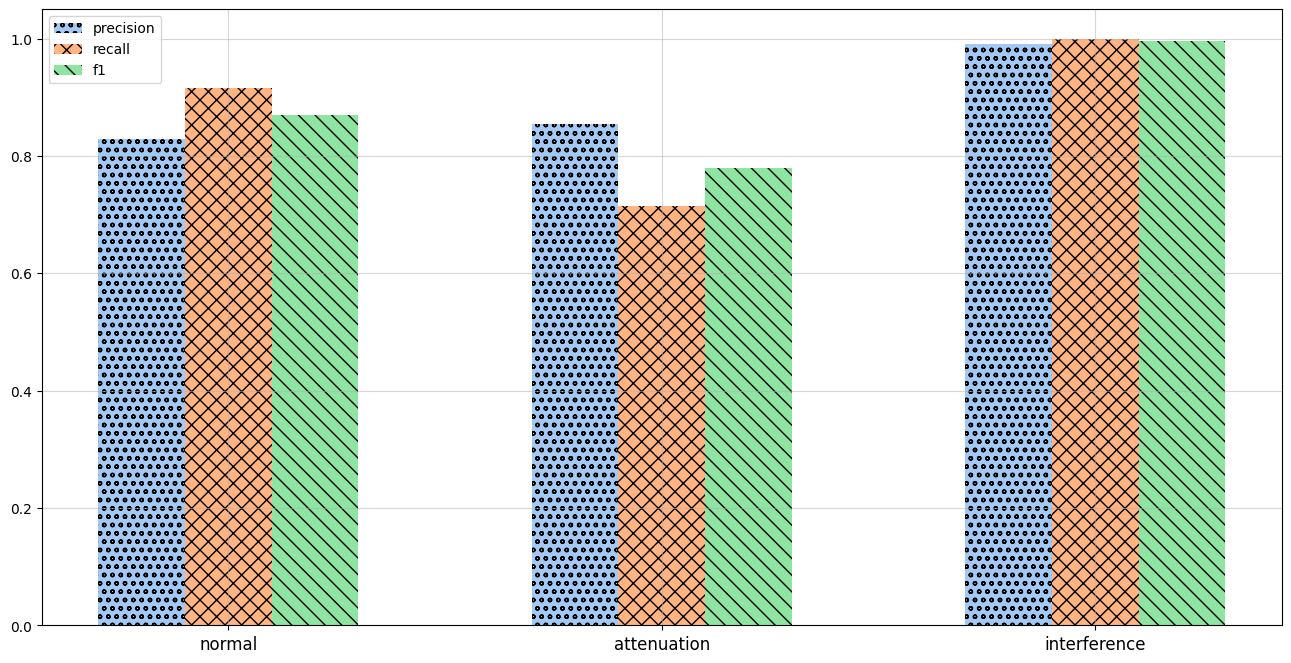
\includegraphics[width=0.5\textwidth]{imgs/chapter_6/per_class_cats.png}
    &
  %\medskip
    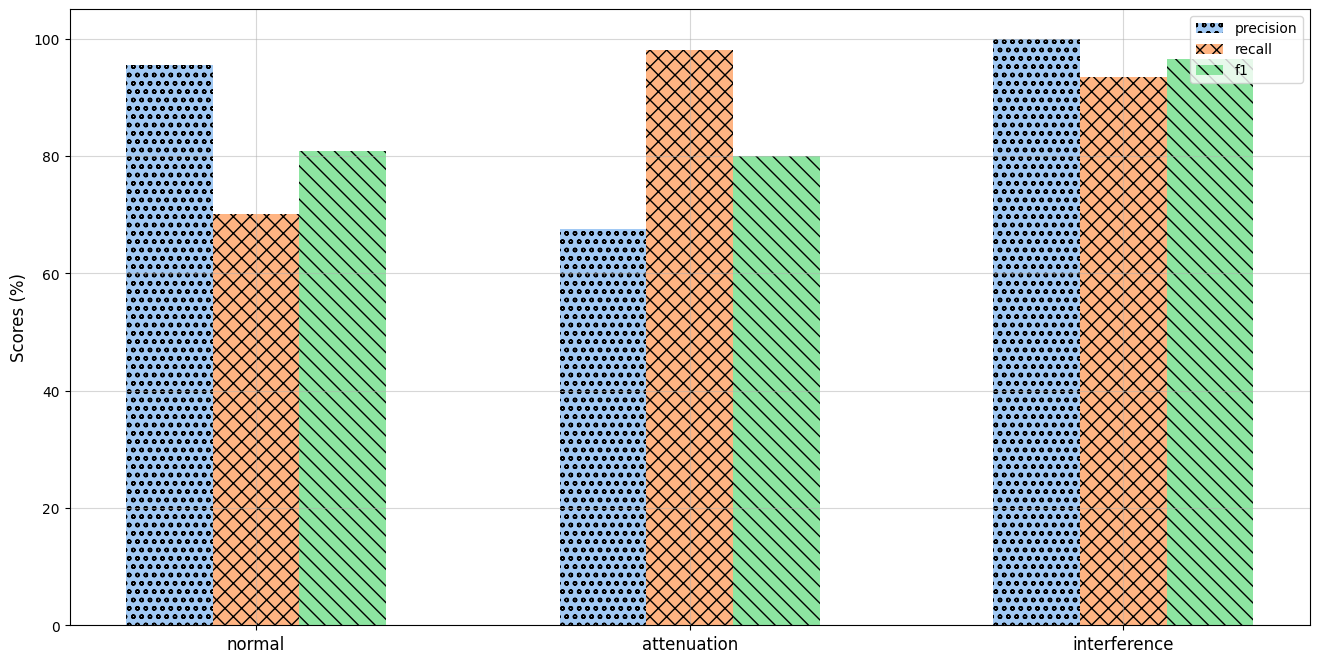
\includegraphics[width=0.5\textwidth]{imgs/chapter_6/per_class_triplet.png}\\
     \small \textbf{(a) RAID} &
    \small \textbf{(b) T-Loss}  \\
  \end{tabular}
  \medskip
  \caption{Per-class precision, recall and F1-score.}
  \label{fig:chap_6:per_class}
\end{figure*}


\subsection{Efficiency with Few Labels}

Fig. \ref{fig:chap_6:finetune_labels} illustrates the evolution of model performance as the percentage of labeled data increases. The left subplot depicts the accuracy scores across various label ratios, while the right subplot presents the corresponding F1-scores.

At the lowest label ratios (1\%-5\%), most models exhibit limited performance, reflecting the inherent difficulty of accurate root cause diagnosis (RCD) with minimal supervision. However, T-Loss and RAID stand out by achieving relatively higher accuracy and F1 scores, showcasing their ability to generalize effectively even with sparse labeled data. T-Loss benefits significantly from its triplet-based pretraining strategy, which efficiently captures meaningful representations from the unlabeled dataset, thereby enhancing fine-tuning performance. Similarly, the pretraining stage of RAID contributes to its robustness in low-label scenarios by effectively leveraging the anomaly detection process to prioritize relevant patterns.

As the label ratio increases, all models demonstrate steady improvement in performance, highlighting the benefits of additional labeled data. Notably, RAID and T-Loss consistently lead in performance, with our solution exhibiting a steady performance boost. This consistency underscores the robustness of RAID across varying levels of supervision. While T-Loss initially competes closely, its performance shows a slight decline between the 5\% and 20\% label ratios, coupled with increased variability, indicating potential sensitivity to the quality or distribution of labeled data in these ranges.

The findings from Fig. \ref{fig:chap_6:finetune_labels} highlight the efficiency of RAID in leveraging limited labeled data, making it an ideal solution for real-world scenarios where labeling is both expensive and time-consuming. Its performance with sparse labels, along with its stable scalability as more labeled data becomes available, firmly establishes RAID as the most suitable model in this evaluation.

\takeaway{RAID also demonstrates strong performance in scenarios with limited labeled data thanks to its anomaly detection stage that effectively prioritize relevant patterns. While T-Loss competes closely in low-label scenarios, its performance exhibits greater variability as label ratios increase.}

\begin{figure*}[!ht]
    \centering
    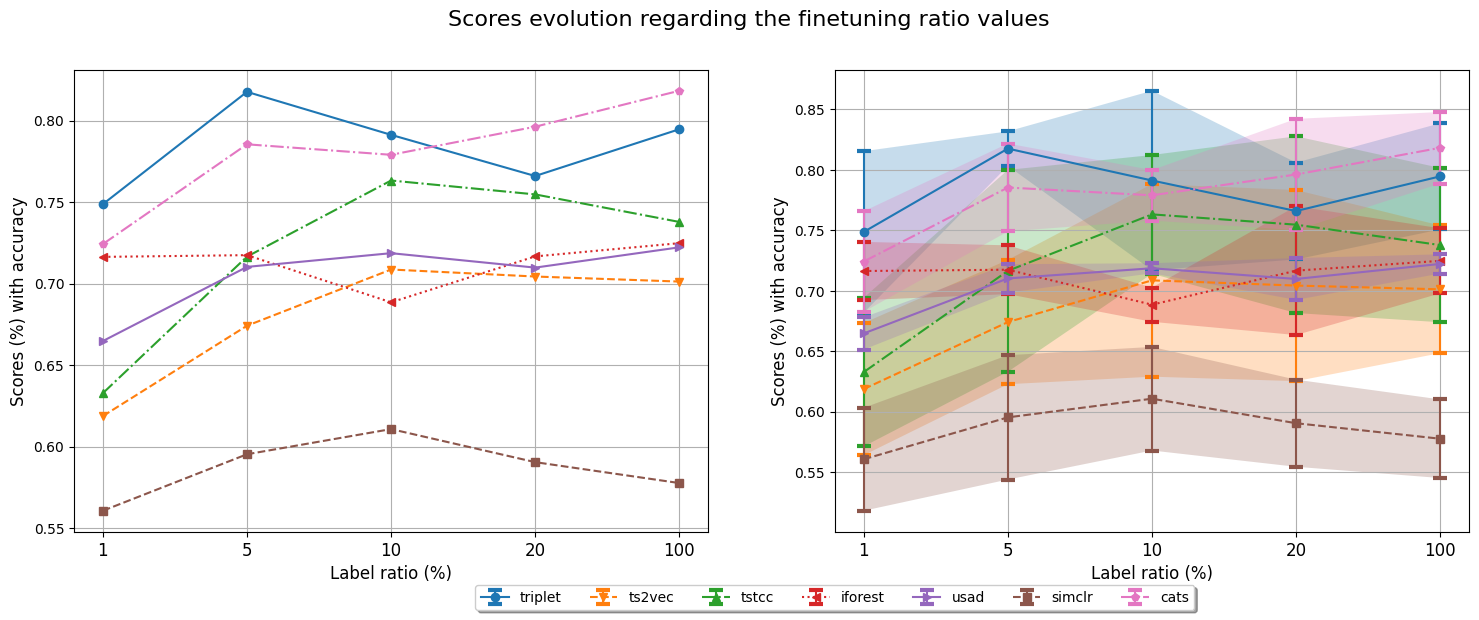
\includegraphics[width=\linewidth]{imgs/chapter_6/labels.png}
    \caption{Performance variation regarding the labels ratio.}
    \label{fig:chap_6:finetune_labels}
\end{figure*}

% On the contrary, models like TS-TCC and SimCLR show significant struggles in this low-label regime, as their reliance on large amounts of labeled data limits their capacity to achieve competitive performance. Similarly, one-stage methods such as T-Loss and TS2Vec exhibit modest improvements but fail to match the performance of two-stage approaches like CATS, which leverage a preliminary anomaly detection stage to guide fine-tuning.

\subsection{Time complexity}

Fig. \ref{fig:chap_6:time_complexity} presents the training time (in seconds) and inference time per time series (in milliseconds) for each of the RCD models. The model with the longest training time is Triplet, which takes approximately 300 seconds, while the fastest training model is 1-NN-DTW, completing training in 500 milliseconds. In terms of inference time, 1-NN-DTW significantly outpaces other models, with the highest inference time of 1800 milliseconds. In contrast, models such as Triplet or TS-TCC, achieve inference times as low as 0.5 milliseconds.

Our proposed solution, RAID, demonstrates a moderate training time of 200 seconds and an inference time of 3.5 milliseconds. While this inference time is the second highest among the models compared, it is still well-suited for real-time deployment, especially in our testbed where data is collected at frequent intervals (e.g., every 3 seconds). This makes RAID an excellent choice for RCD, as it balances moderate training overhead with sufficiently low inference latency, allowing for continuous monitoring and fast anomaly detection. Additionally, being a two-stage model, RAID offers a key advantage: when new causes or anomalies are detected, only the supervised classifier requires retraining. Most of the training time originates from the initial anomaly detection phase, unlike one-stage models that require complete retraining, including the pretraining phase. This makes RAID more efficient for scenarios requiring periodic updates or retraining, reducing overall downtime and resource consumption.

In summary, RAID strikes a practical balance between training efficiency and inference speed, making it highly effective for real-time RCD in dynamic and large-scale network environments.


\takeaway{RAID achieves a practical balance between training efficiency and inference speed, with a training time of 200 seconds and an inference time of 3.5 milliseconds. RAID's two-stage design further enhances its practicality by requiring retraining only for the supervised classifier when new anomalies are detected, unlike one-stage models that necessitate full retraining.}

\begin{figure*}[!ht]
    \centering
    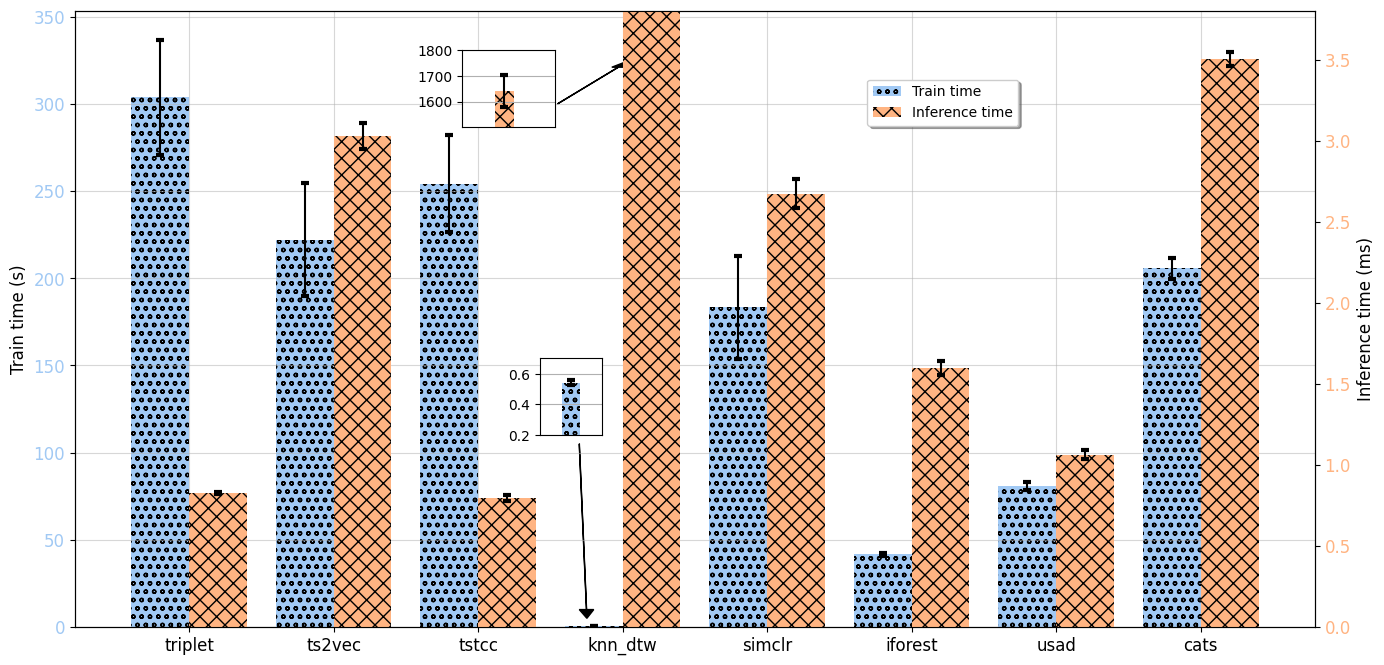
\includegraphics[width=\linewidth]{imgs/chapter_6/time.png}
    \caption{Time complexity of each model.}
    \label{fig:chap_6:time_complexity}
\end{figure*}

\section{Conclusion and Future work}\label{chap_6:conclusion}
This chapter presented a Root Cause Diagnosis (RCD) approach for identifying network issues in Cloud VR sessions over Wi-Fi networks, utilizing time series KPIs collected from access points. By employing a two-stage framework, we demonstrated the effectiveness of our approach compared to traditional time series classification methods. Our proposed architecture, which integrates contrastive learning into the anomaly detection process, has shown significant improvements in both identifying anomalies and diagnosing the root causes of Cloud VR performance issues. This provides a good foundation for future research in real-time diagnostics for cloud-based VR applications. One key strength of this approach is its balance between training time and inference speed, making it ideal for real-time diagnostics in dynamic network environments. Moreover, the two-stage design enhances efficiency by isolating retraining to the supervised classifier, thus avoiding full model retraining when new causes are introduced.

Despite the promising results, there are several areas that warrant further exploration and improvement. First, while our model performs well in detecting clear anomaly patterns such as interference, its sensitivity to more nuanced variations—particularly in attenuation scenarios—needs to be enhanced. Future work will focus on improving the model’s ability to detect subtle transitions between normal and degraded states. Second, scaling the solution to larger and more complex datasets is a priority. Our current framework has been tested on a controlled Cloud VR testbed with only two types of impairments. To improve its robustness, future research should include additional Wi-Fi impairments such as network congestion, hidden terminal issues, and non-Wi-Fi interference. Expanding the test environment to include more diverse real-world conditions, such as home networks where multiple sources of impairments may coexist, will also offer valuable insights. Finally, extending this two-stage model to a multi-modal diagnostic approach could provide a more comprehensive view of the root cause diagnosis process. By incorporating additional data sources, such as application-level performance metrics or raw network PCAP data, the system could offer even more accurate and proactive detection of network impairments. These enhancements will be crucial for addressing the growing demands of next-generation low-latency applications like Cloud VR.